\section{题目二}
\subsection{实验目的}
安装配置UNIX V6++的调试环境。
\subsection{实验内容}
\begin{enumerate}
    \item 启动UNIX V6++的调试模式;
    \item  利用本地VSCODE进行远程调试。
\end{enumerate}
\subsection{实验过程}
由于无法正常启动远程桌面环境中的Vscode,所以利用本地Vscode进行调试。首先在远程界面环境中执行make qemug命令,然后再本地Vscode中连接远程桌面环境,
并打开unix-v6pp-tongji文件夹。接着将调试对象设置为内核,并在next函数中设置断点。在Vscode中开始调试并命中断点后,进行单步调试,直至内核初始化完成。
\begin{figure}[!htbp]
    \centering
    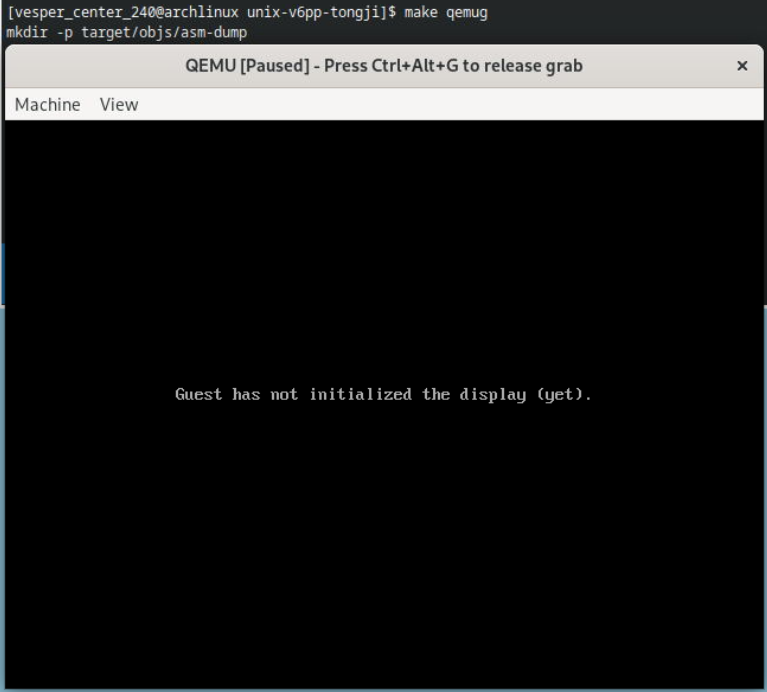
\includegraphics[scale=0.5]{fig/qemug.png}
    \caption{执行make qemug命令}\label{qemug}
\end{figure}

\begin{figure}[!htbp]
    \centering
    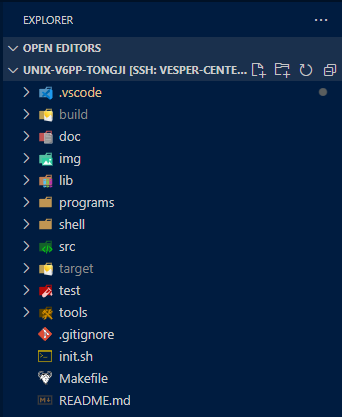
\includegraphics[scale=1]{fig/folder.png}
    \caption{打开unix-v6pp-tongji文件夹}\label{folder}
\end{figure}

\begin{figure}[!htbp]
    \centering
    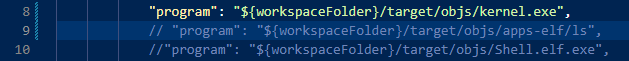
\includegraphics[scale=1]{fig/kernel.png}
    \caption{设置调试对象}\label{kernel}
\end{figure}

\begin{figure}[!htbp]
    \centering
    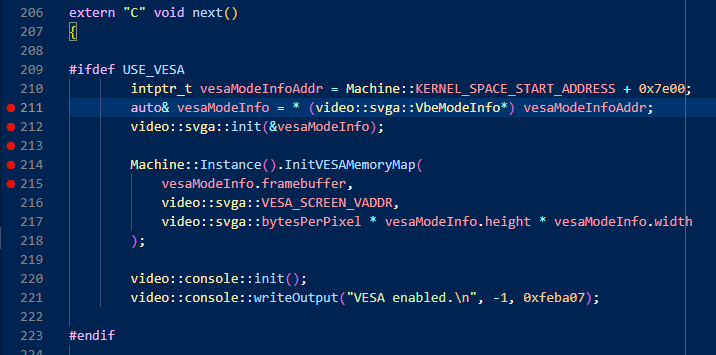
\includegraphics[scale=0.7]{fig/breakpoint.png}
    \caption{设置断点}\label{breakpoint}
\end{figure}

\begin{figure}[!htbp]
    \centering
    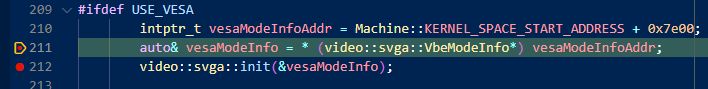
\includegraphics[scale=0.7]{fig/hit.png}
    \caption{命中断点}\label{hit}
\end{figure}

\begin{figure}[!htbp]
    \centering
    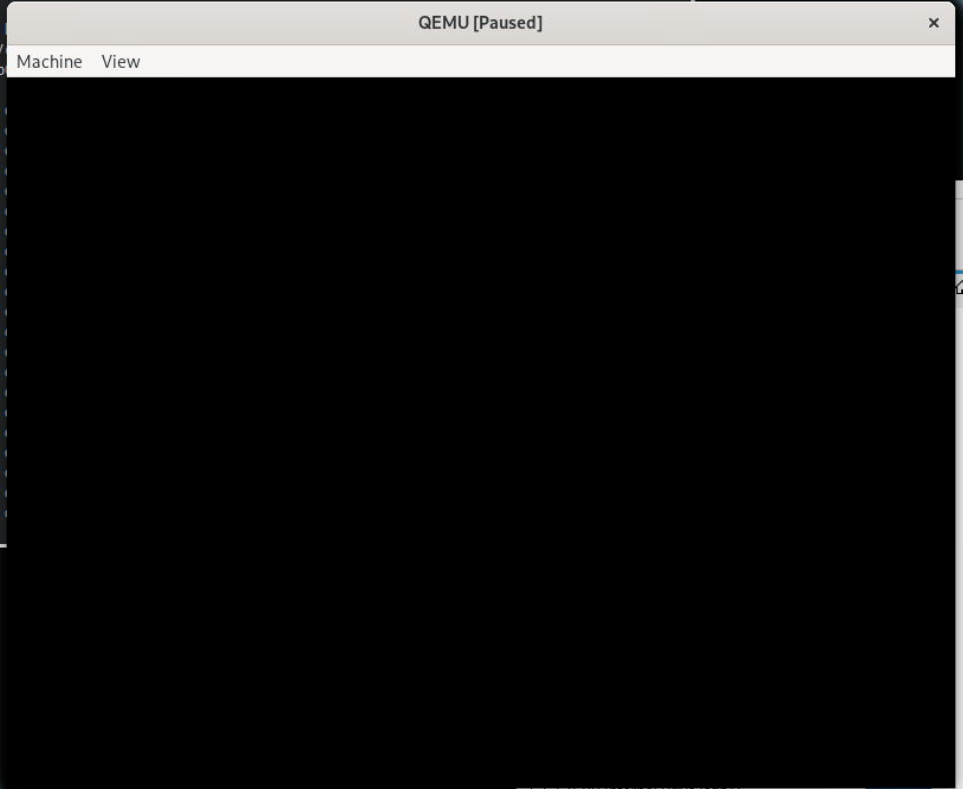
\includegraphics[scale=0.5]{fig/hitScreen.png}
    \caption{命中断点时的界面}\label{hitScreen}
\end{figure}

\begin{figure}[!htbp]
    \centering
    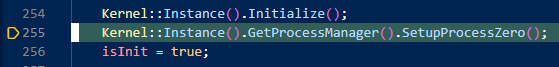
\includegraphics[scale=1]{fig/stepOver.png}
    \caption{单步调试}\label{stepOver}
\end{figure}

\begin{figure}[!htbp]
    \centering
    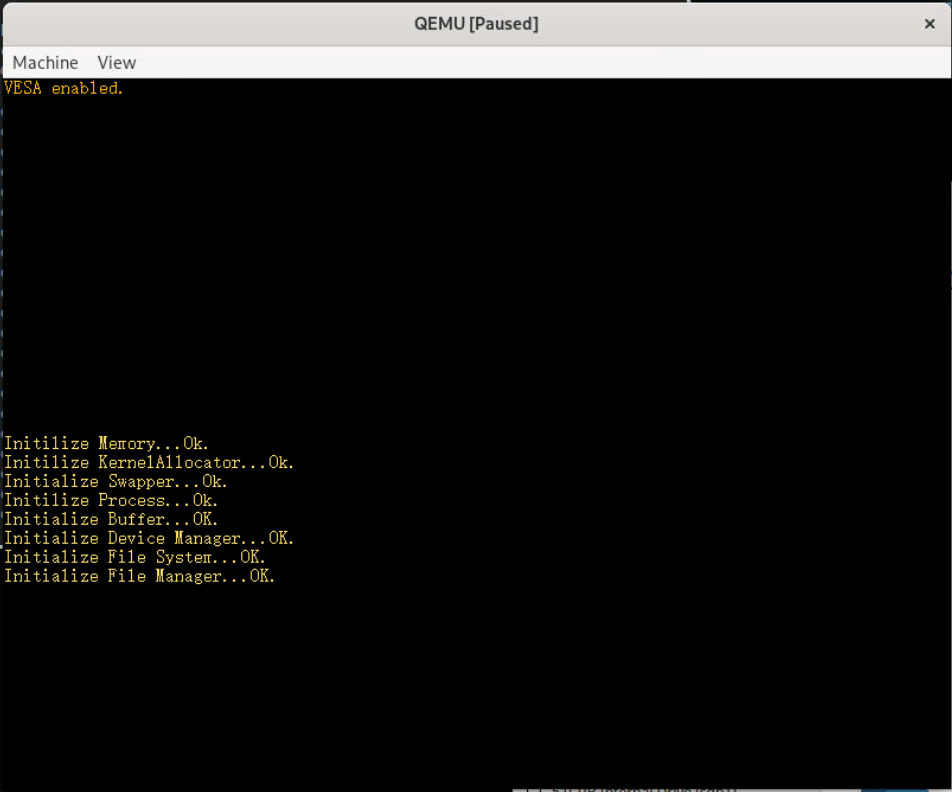
\includegraphics[scale=0.5]{fig/initialized.png}
    \caption{内核初始化完成时的界面}\label{initialized}
\end{figure}


